\subsection{PlayerList}

\begin{figure}[H]
    \centering
    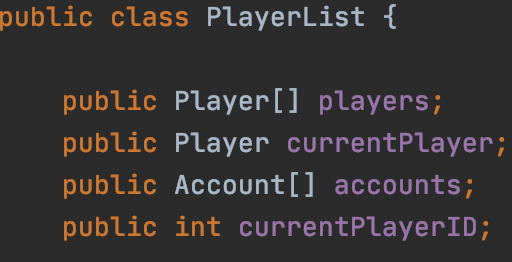
\includegraphics[width=\textwidth]{sources/7_implementering/PlayerList Properties.png}
    \caption{PlayerList Properties}
    \label{fig:plProps}
\end{figure}
Playerlisten bruges til at oprette spiller-arrayet, så hver spiller kan få sin tur i spillet. Playerlisten bliver oprettet efter man vælger antallet af spillere, som er med i spillet. Der bliver her oprettet et nummer for hver spiller, og accountet tilhørende hver spiller bliver sammensat.
\begin{figure}[H]
    \centering
    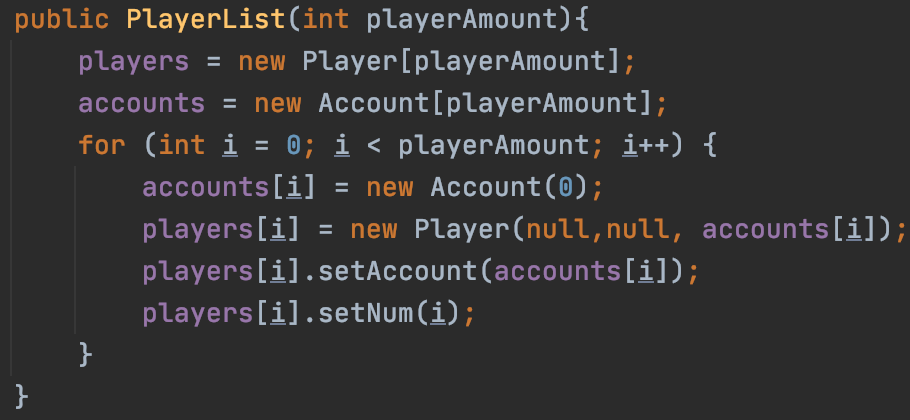
\includegraphics[width=\textwidth]{sources/7_implementering/PlayerList PlayerList.png}
    \caption{PlayerList metode}
    \label{fig:plMetode}
\end{figure}
Efter dette har vi getters og setters til at holde styr på mængden af spillere og vores PlayerList. Vi kan bl.a. få fat i mængden af spillere samt få fat i den nuværende spiller og næste spiller. Dette bruges blandt andet i logikken, når den nuværende spiller tager sin tur, og når turen er færdig og spillet skal have fat i den næste spiller.
\begin{figure}[H]
    \centering
    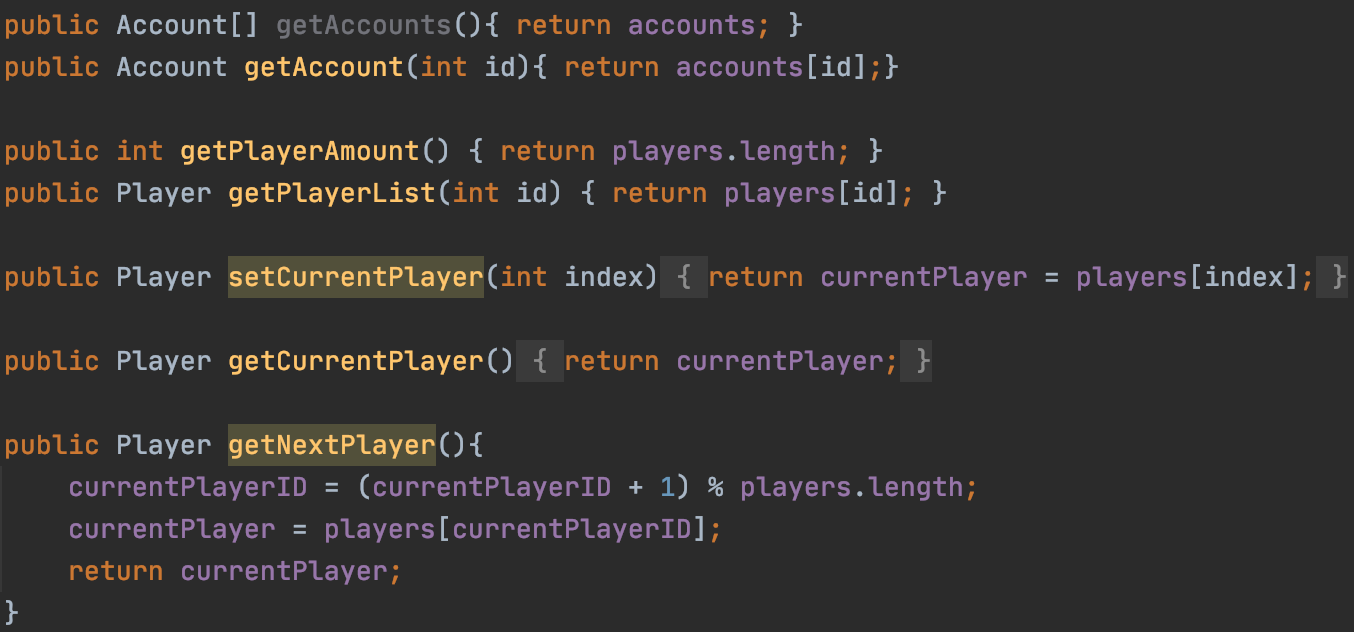
\includegraphics[width=\textwidth]{sources/7_implementering/PlayerList Getters Setters.png}
    \caption{Playerlist Getter/Setter}
    \label{fig:plGetSet}
\end{figure}